\begin{figure}
    \centering
    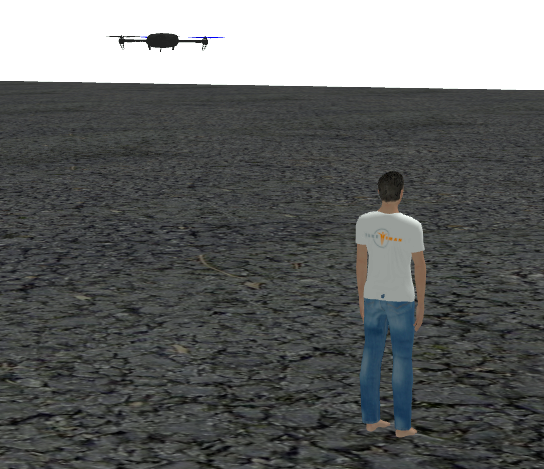
\includegraphics[width=0.4\textwidth]{images/screen_simulazione.png}
    \caption{Simulation's SITL image.}
    \label{SOL:fig:screensimulazione}
\end{figure}

\subsection{ROS2 Brief introduction}
Before diving into the simulation, is important to explain the ROS2 functioning. The Robot Operating System (ROS) is a set of software libraries and tools for building robot applications. A ROS2 application, can be seen as a network, or better a graph, composed by ROS2 elements, processing together at the same time. The principal ROS2 elements are the nodes, which are the actual computational elements. Each node can send and receive data from other nodes via topics, services, actions, or parameters. ROS2 Nodes can be software Robotic components, like the Flight controller, or can be user programmed. The base principle in ROS2 nodes communication is the pubblisher/subscriber protocol. For what concerns topics (which are the only communication medium used in this work), each node can be a publisher, so it can "change" the topic value, or a subscriber, so it can "read" the topic value. In this way, ROS2 is an effective communication interface between different hardware and software, with the only requirement of being connected to the same network. A representation example of a ROS2 network, is the one of our Simulation depicted and explained in \autoref{SIM:fig:nodism}.\\
A user programmed Node is typically defined inside the so called ROS2 packages, in which the Node executable can be interfaced with user defined topics and messages, or with some defined by others. For example the PX4 team have developed a series of packages in which they define all the messages topics, services and actions needed to fully interact with the flight controller (regardless if it is the simulated one or a real one, since they are equal in software). Packages can be programmed both in C++ or Python, and can be grouped together in ROS2 workspace. For better details, we refer to the ROS2 Documentation\cite{ros2doc}.

\begin{figure}
    \centering
    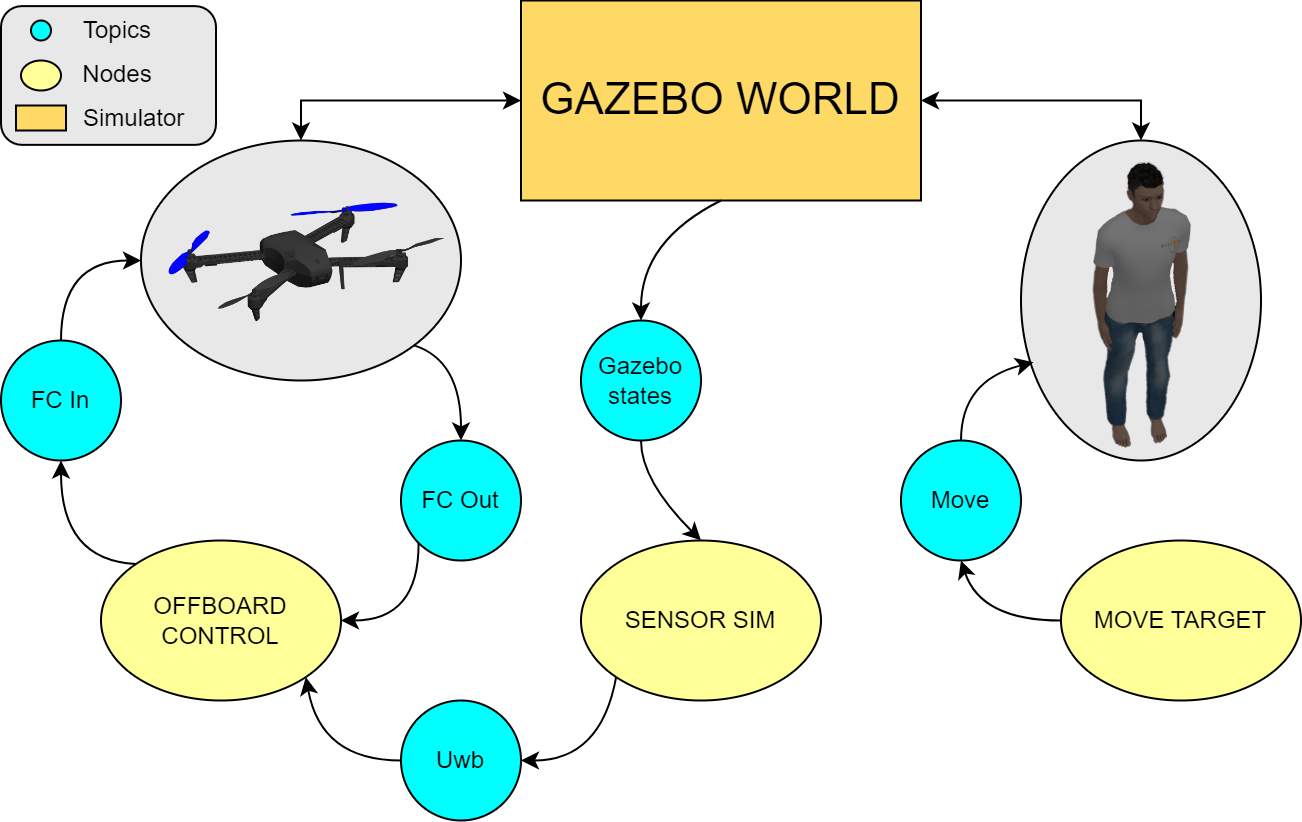
\includegraphics[width=0.45\textwidth]{images/nodi_simulazione.png}
    \caption{ROS2 simulation Network. The nodes (yellow ellipses) can be subscriber or publisher to the topics (light blue circles). In this way, for example, the offboard node can retrieve the drone's state estimates from the FC, and send to it the controls.}
    \label{SIM:fig:nodism}
\end{figure}

\subsection{Simulation}
To assess and validate the developed control law, is necessary to test it on a simulation that well resembles the reality.
This is possible conducting software in the loop simulations, with the same flight controller available as hardware and possibly with the same vehicle.
Working with the PX4 flight stack, as it is the one that runs on our flight controller, the best simulation environment to use is Gazebo, a graphic simulator with an accurate physics. It is also easily customizable through the use of plugins permitting to include other effects as the wind. Moreover, it interacts well with ROS2,  allowing for a lot of flexibility in use.\\
The vehicle on which we tested our control law in simulation is the Iris quadcopter, the main model for gazebo PX4 simulations (even though it is different from the one we used in real tests). This model guarantees a great level of simulation accuracy: the motors and the generated thrusts are modelled accurately using specific plugins, and even its navigation sensors are corrupted appropriately to be similar to real-case scenarios. Even the flight controller is simulated as the real one, having the same estimation algorithms, controller and characteristics.\\
To simulate the target we defined a simple object, with the appearance of a human, that can translate in the x and y direction. To make it move, we created a ROS2 node that publishes on the gazebo ROS2 topics the position of the target, making it move. To make it move at a certain speed and with the desired trajectory, nearby points are sent to gazebo at a constant rate.\\
To simulate the range and AoA sensor, it is necessary to know the global position in the gazebo world of both target and drone, together with the yaw of this last one. Once that these information are known, and in our case it is simply done with another ROS2 node that subscribes to the pose topic of the objects in gazebo, with simple geometric relations it is possible to determine the true angle and range and then corrupt them with noise, to simulate the sensor. In our simulations, we simply added normally distributed, zero mean and white noise to both quantities (referring to the values obtained in the characterization of the true sensor). This simulated sensor node, supplies the simulated sensor readings to the offboard-control node which, by accessing to the drone estimates, compute the velocity setpoints as in \eqref{PF:VELxy}, together with the yaw setpoint \eqref{PF:yawsp} and the position setpoint for the height control, sending them to the FC. It is interesting to note that, since the flight controller is fed via ROS2 even in the real case, the same offboard control node can be used in the real application, of course using the range and AoA measures given by the real UWB sensor. A Detailed scheme of the ROS2 network is presented in \autoref{SIM:fig:nodism}. Simulation results are exposed later, in \autoref{SIM_RES}.